\documentclass[12pt]{report}
\usepackage[T1]{fontenc}
\usepackage[french]{babel}
\usepackage[utf8x]{inputenc}
\usepackage{amsmath}
\usepackage{graphicx}
\usepackage[colorinlistoftodos]{todonotes}
\usepackage[strings]{underscore}
\usepackage{url}
\usepackage{hyperref}
\hypersetup{%
    pdfborder = {0 0 0}
}

\begin{document}



%-----------------------------------------------------------------%
%    PAGE DE TITRE
%-----------------------------------------------------------------%

\begin{titlepage}

\newcommand{\HRule}{\rule{\linewidth}{0.7mm}} % Trait horizontal

\center
 
%---------------------------%
%   LOGO & EN-TÊTE DE PAGE
%---------------------------%

\includegraphics[width=0.8\textwidth]{img/logo.jpg}\\

\textsc{\Large Projet de Programmation}\\[0.5cm]
\textsc{\large Génération procédurale de planètes}\\[0.5cm]

%---------------------------%
%   TITRE
%---------------------------%

\HRule \\[0.4cm]
{ \huge \bfseries Cahier des besoins}\\[0.4cm]
\HRule \\[1.5cm]
 
%---------------------------%
%   AUTHEURS
%---------------------------%

\begin{minipage}{0.4\textwidth}
\begin{flushleft} \large
\emph{Auteurs:}\\
Rémy \textsc{Maugey}\\
Jérémi \textsc{Bernard}\\
Hugo \textsc{Alonso}\\
Brian \textsc{Mazé}\\
\end{flushleft}
\end{minipage}
~
\begin{minipage}{0.4\textwidth}
\begin{flushright} \large
\emph{Client:} \\
Emmanuel \textsc{Fleury}
\end{flushright}
~
\begin{flushright} \large
\emph{Chargé de TD:} \\
Boris \textsc{Mansencal}
\end{flushright}
\end{minipage}\\[2cm]

%---------------------------%
%   DATE
%---------------------------%

{\large \today}\\[2cm] 


\vfill % Fill the rest of the page with whitespace

\end{titlepage}
%-----------------------------------------------------------------%
%   FIN PAGE DE TITRE
%-----------------------------------------------------------------%

%-----------------------------------------------------------------%
%   Table des Matières
%-----------------------------------------------------------------%


\tableofcontents

\thispagestyle{empty} % empeche l'affichage du numero de cet page

%-----------------------------------------------------------------%
%   Introduction
%-----------------------------------------------------------------%

\newpage

\chapter*{Introduction}
\addcontentsline{toc}{chapter}{Introduction}
\setcounter{chapter}{1}

L'objectif de ce projet est de générer le terrain (voir figure
\ref{fig:terrain}) d'une planète procéduralement et de l'afficher à
l'écran.

\begin{center}
\begin{figure}[!h]
  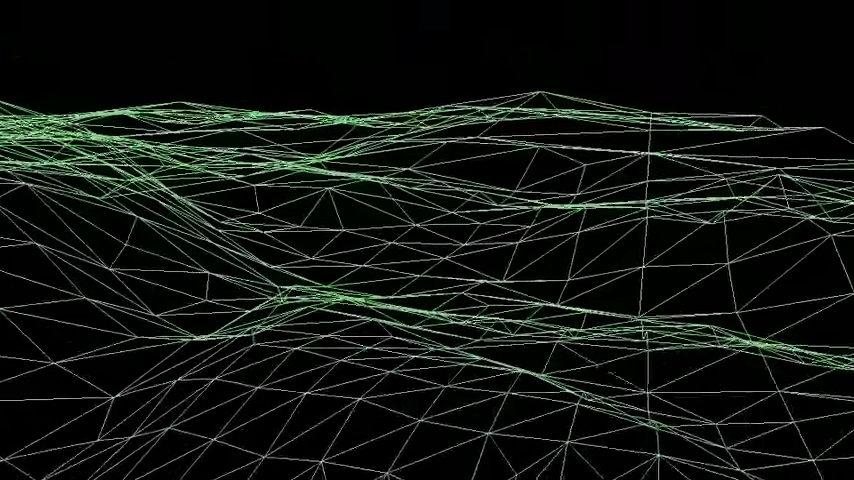
\includegraphics[scale=0.5]{img/terrain.png}
  \caption{Terrain procédural\protect\footnotemark}
  \label{fig:terrain}
\end{figure}
\end{center}

%Parce que latex
\footnotetext{Source: \url{https://youtu.be/AT7h8pYJRiw}}
Une planète en trois dimensions complexe est un ensemble de sommets reliés
entre eux par des arrêtes, formant des faces triangulaires regroupées grille appelé maillage.\\
Le nombre d'images par seconde affichable à l'écran étant directement proportionnel aux nombre de sommets et de triangle, il est rapidement nécessaire d'avoir recourt à des méthodes d'optimisation.
%Ces triangles sont ensuite
%traités et affichés à l'écran en deux dimensions. Plus le nombre de
%triangles à afficher est élevé, plus le rendu d'une image est long, ce
%qui est problématique dans une application nécessitant de générer
%beaucoup d'images rapidement, par exemple pour un rendu temps réel dans
%une simulation ou un jeu vidéo.\\
Il est alors intéressant de pouvoir réduire le nombre de triangles d'un
objet qui n'a pas besoin d'être très détaillé dans un cas précis, par
exemple si l'objet est loin de l'observateur. Un cas particulier est
l'affichage d'une surface très grande comportant des aspérités, par
exemple un terrain. Une partie du terrain est proche de l'observateur,
nous voulons donc en afficher les détails, mais une autre partie est
plus éloignée, et les détails seront moins visibles sur l'image finale.
On peut donc réduire le nombre de triangle de la partie éloignée afin de
réduire le nombre de triangles à traiter. Pour simplifier le stockage
des données du terrain, on peut représenter les points du maillage
uniquement par leur hauteur par rapport au rayon de la sphère. Un
tableau représentant la hauteur d'un ensemble de points reliés est
appelé carte de hauteur ou \emph{heightmap}.

Le but est donc d'implémenter un système de \emph{LOD} (
\emph{Level of Detail}: niveau de détail) à appliquer sur le maillage
d'une sphère en vue d'une application en temps interactif, afin
d'optimiser son affichage. Le projet comportera une application
permettant le rendu de cette sphère en trois dimensions, afin de pouvoir
visualiser le fonctionnement du système de \emph{LOD}, ainsi qu'un moyen
de mesurer les performances du système.

%-----------------------------------------------------------------%
%   État de l’existant
%-----------------------------------------------------------------%
\newpage

\chapter*{État de l'existant}
\addcontentsline{toc}{chapter}{État de l'art}
\setcounter{chapter}{2}

De nombreuses applications utilisent des techniques d'optimisation de
l'affichage. Notamment les applications qui demandent de bonnes
performances tel que les simulations 3D ou les jeux vidéos.
%Génération Procédural
Dans le cas du développement d'un environnement 3D il est souvent fait
appel à des techniques de génération procédural, par exemple le logiciel
Terragen\footnote{Terragen: \url{http://planetside.co.uk/}} comme
présenté en figure \ref{fig:Terragen} qui est utilisé dans le monde du
cinéma ou encore Elite Dangerous\footnote{Elite Dangerous:
\url{https://www.elitedangerous.com/}} dans le monde du jeux vidéos.
Ces deux applications utilisent des mécanisme de génération procédurale
pour créer respectivement des planètes et une galaxie.

%LOD et dérivé
Plusieurs algorithmes peuvent être utilisé dans la mise en place d'un
système de niveau de détail dynamique, tous d'abord le \cite{CDLOD} qui
est utilisé comme référence dans le cadre de se projet.  Il a l'avantage
de rattacher les maillages des différents niveaux de détails de manière
lisse et progressive c'est à dire sans frontières intermédiaires,
empêchant l'apparition de discontinuités.  Un autre avantage de cette
méthode est de garder le nombre de triangles affichés constant, en
répartissant les triangles dans les différents niveaux de détails.\\
Du code d'exemple est fournit par l'auteur du papier de référence,
cependant il utilise la bibliothèque graphique DirectX. Il est
uniquement compatible avec Windows et ne peut pas être utilisé tel quel
dans notre projet.  Pour être compatible avec le système d'exploitation
cible, il est nécessaire d'utiliser la bibliothèque graphique OpenGl à la
place. De plus, les algorithmes utilisé comme base par \cite{CDLOD} sont
implémentés sur \emph{GPU}.  Une autre approche serait de mettre à jour
des zones entière de terrain, comme détaillé par \cite{MassiveTerrain}.
Cet algorithme ne permet pas de garder un nombre constant de triangles
affichés par le fait qu'ils s'affichent par groupe. Il est aussi
implémenté sur \emph{GPU}.\\
L'algorithme de CDLOD a déjà été implémenté dans \cite{WorldGenerator}.
\cite{WorldGenerator} est implémenté en C++, l'algorithme est
réutilisable. La partie rendue est écrite en shaders OpenGL.

On peut voir que la plupart des algorithmes modernes sont développés
sur \emph{GPU}.  En effet, la possibilité de développer au sein d'une
carte graphique remonte à environ 1995 comme on peut le voir dans
\cite{EvoGPU}. Notre objectif ici est de montrer à quelle point les
processeurs moderne sont capables de faire ce même travail.

\begin{center}
\begin{figure}[!h]
  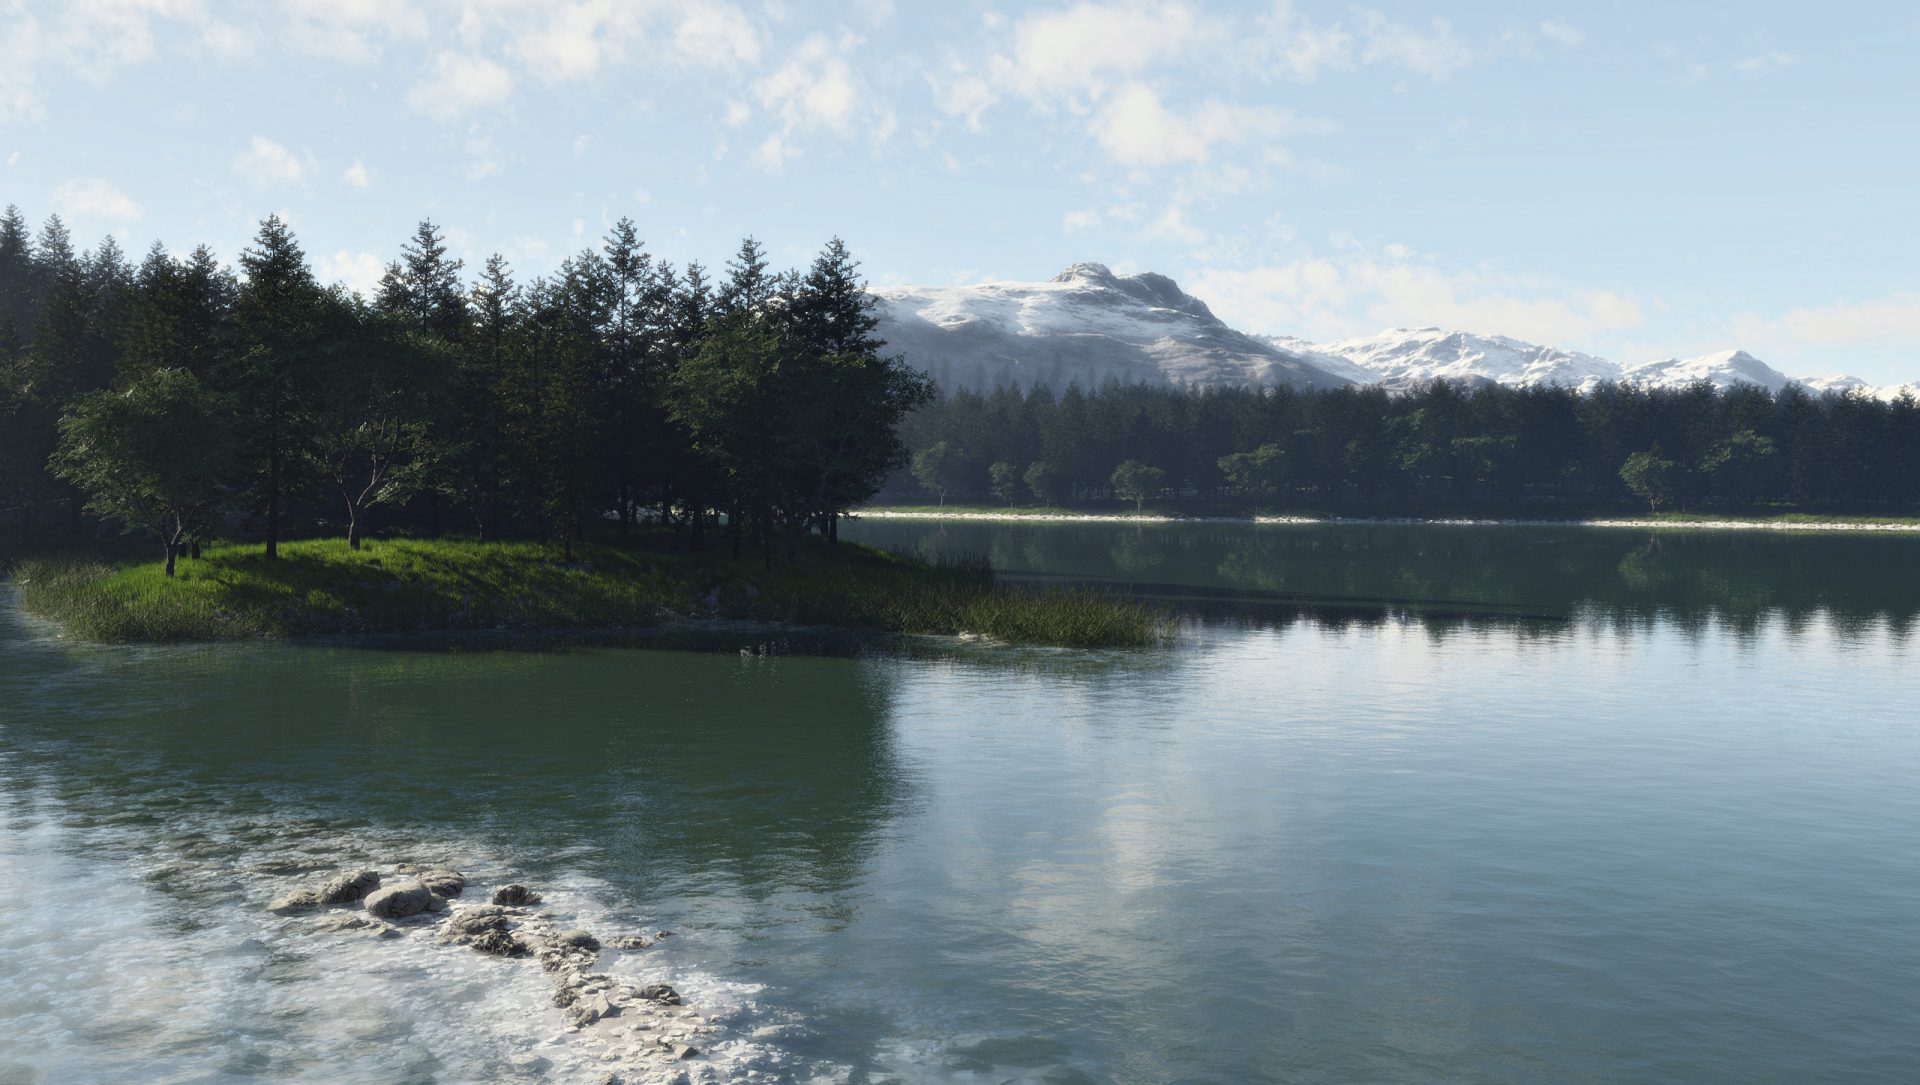
\includegraphics[scale=0.2]{img/Lake.jpg}
  \caption{Terragen: \protect\url{http://planetside.co.uk/}}
  \label{fig:Terragen}
\end{figure}
\end{center}

%-----------------------------------------------------------------%
%   ANALYSE DES BESOINS
%-----------------------------------------------------------------%
\newpage

\chapter*{Analyse des besoins}
\addcontentsline{toc}{chapter}{Analyse des besoins}
\setcounter{chapter}{3}

%---------------------------%
%   BESOINS FONCTIONNELS
%---------------------------%

\section{Besoins fonctionnels}

\subsection{Interface graphique}

L'interface sera implémentée avec OpenGL 3.3 et ciblant Linux.\\
Afficher à l'écran une scène en trois dimensions représentant la planète.\\
La surface de la planète sera affichée en maillage, afin de bien voir
les triangles créés par l'algorithme.\\
Déplacer la caméra dans l'espace en fonction des entrées clavier et
souris de l'utilisateur.\\
Afficher dans un coin de l'écran les informations sur les performances
sous forme du nombre d'images par seconde.\\

Cette partie a une priorité haute car nécessaire pour tester les
algorithmes. Cette partie est séparable en plusieurs sous parties:
\begin{itemize}
  \item Création de la fenêtre
  \item Génération de la sphère
  \item Génération du maillage
  \item Affichage dans la scène 3D
\end{itemize}
Nous estimons le temps nécessaire à cette partie à deux semaines.

\subsection{Génération de terrain}


Générer aléatoirement la carte de hauteur d'un terrain.  La génération
se fera à partir d'un algorithme d'un bruit Simplex 3D déjà implémenté
dans une dépendance, par exemple \cite{libnoise}. Ce type d'algorithme
est souvent utilisé dans le cadre de génération procédurale pour son
efficacité. Plusieurs algorithmes de bruits sont disponibles, cependant
le bruit Simplex est plus performant dans un nombre plus élevé de
dimensions \cite{Simplexnoise}.  Pour former la sphère, il suffit de
construire un cube quadrillé et de le déformer en sphère (voir figure
\ref{fig:Cubetosphere} ), en utilisant les formules de
\cite{Cube2Sphere}. Cette technique est adaptable à notre projet, car
c'est celle utilisée dans \cite{WorldGenerator}. Elle permet de garder
des découpages carrés, ce qui simplifie les opérations dans le
quadtree.\\

\begin{center}
\begin{figure}[!h]
  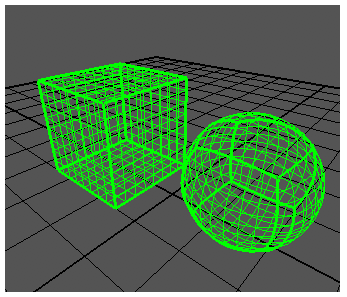
\includegraphics[scale=1]{img/Cubetosphere.png}
  \caption{Transformation d'un cube en sphère \cite{Cube2Sphere}}
  \label{fig:Cubetosphere}
\end{figure}
\end{center}

Priorité moyenne, le terrain généré est nécessaire aux tests de
l'interface graphique et des algorithmes, mais n'est pas requis pour
commencer leurs développements. Cette partie se découpe en:
\begin{itemize}
  \item Génération de la carte de hauteur
  \item Appliquer la carte de hauteur sur la maillage
\end{itemize}
Le temps de développement est estimé à une semaine.

\subsection{Structure de donnée}

Implémenter une structure de donnée représentant un quadtree pour
l'algorithme de CDLOD (voir figure \ref{fig:quadtree} tirée de 
\cite{CDLOD}).\\
Un quadtree est un arbre dont chaque nœud possède quatre fils, cette
structure de donnée nous permet de subdiviser le terrain, chaque nœud
représentant une surface du terrain. Une nœud contient la représentation
de sa zone à son niveau de détail, et quatre fils représentant chacun un
quart de la zone du parent au niveau de détail supérieur.\\
La hauteur de l'arbre représente le nombre de niveau de détail.
La structure de donnée est fixe et paramétrable.
\begin{center}
\begin{figure}[!h]
  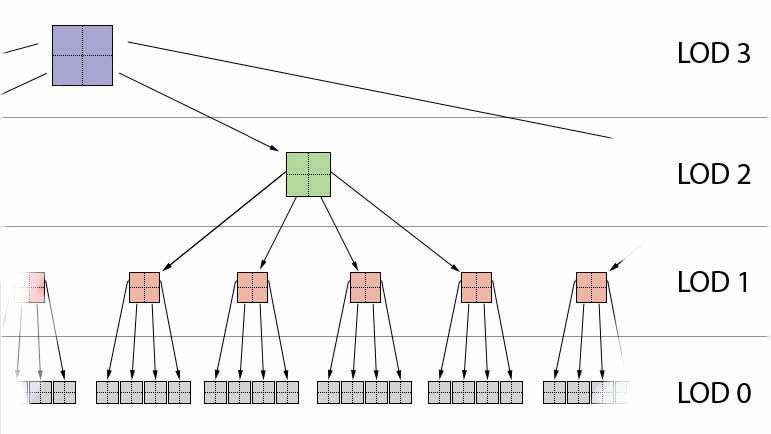
\includegraphics[scale=0.5]{img/Quadtree.png}
  \caption{quadtree \cite{CDLOD}}
  \label{fig:quadtree}
\end{figure}
\end{center}

La structure de donnée est la base de l'algorithme de CDLOD. Elle est
donc de haute priorité. Nous estimons la durée de développement à deux
semaines.\\

\subsection{CDLOD}

Implémenter un algorithme inspiré de \cite{CDLOD}, conformément aux
demandes du client.  L'algorithme permettra de générer les différents
niveaux de détails de la surface de la planète, et sera accessible dans
une bibliothèque séparée du reste du projet. La structure de donnée et
les algorithmes correspondant seront fournis indépendamment de la partie
affichage graphique dans une interface de programmation.\\
L'API peut être vue comme une base de donnée, des requêtes sont faites
en lui donnant le frustum de la caméra, c'est à dire son cône de vision,
ainsi que ses informations tel que les coordonnées.

La bibliothèque retournera un arbre composé des différentes cartes de
hauteurs.\\

Les distances auxquelles les transitions entre deux niveaux de détail
ont lieu seront choisies après expérimentation. Idéalement, les
transitions sont plus longues sur les niveaux les moins détaillés.

\begin{center}
\begin{figure}[!h]
  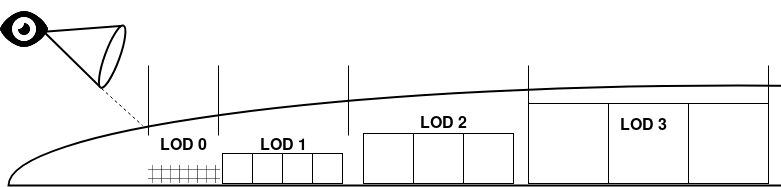
\includegraphics[scale=0.5]{img/lods.png}
  \caption{Différents niveaux de détails en fonction de la distance à la
  caméra}
  \label{fig:lods}
\end{figure}
\end{center}

L'algorithme de CDLOD est de priorité moyenne car nécessite
l'implémentation de la structure de donnée en premier. Son
développement prendra trois semaines selon nos estimations.\\

\subsection{Mesure des performances}

Mesurer le nombre d'images générées par seconde, les afficher à
l'écran.\\
Mesurer le temps de réponse de la bibliothèque à chaque requête.\\
Afficher les résultats dans la sortie standard à la fin de l'exécution
du programme.\\

Les tests de performance sont de priorité faible. Il seront implémenté
en dernier. Nous estimons que leur développement prendra une semaine.\\

%---------------------------%
%   BESOINS NON FONCTIONNELS
%---------------------------%

\newpage
\section{Besoins non fonctionnels}

\subsection{Structure de donnée}

Les cartes de hauteur seront stockées dans des tableaux de flottant à
deux dimensions. Ainsi cela nous laisse une certaine marge de manœuvre
sur la précision des hauteurs. Chaque hauteur prendra donc 4 octets dans
la mémoire vive. Nous estimons que la taille total de l'arbre dans la
mémoire sera de l'ordre de la centaine de Mo.\\


\subsection{Performances}

L'objectif du projet étant de tester les performances d'une
implémentation de \cite{CDLOD}, il n'y a pas de contrainte de
performance imposées par le client. Nous pouvons prévoir grâce aux
études de performances de \cite{CDLOD} l'impacte de performance de
l'algorithme de CDLOD. Sur des processeurs performants de l'époque,
\cite{CDLOD} mesure en moyenne 0.08ms de temps de parcours de l'arbre
nécessaire pour générer le maillage du terrain. A cela devront s'ajouter
les coups de génération du maillage, ainsi que les coups de rendu de la
scène.  Pour un rendu très fluide, lorsque la caméra se
déplace dans la scène, il faudrait atteindre au moins 60 images par
secondes, donc passer moins de 16ms de calcul par image. \cite{CDLOD}
atteint des performances élevées en effectuant une partie des calculs de
la scène sur GPU.  Des algorithmes similaires à \cite{CDLOD} comme
\cite{PlanetRenderer} atteignent plusieurs centaines d'images par
secondes.\\
Comme notre implémentation sera largement sur CPU, nos
performances seront plus faibles, cependant les mesures de performances
de \cite{CDLOD} sur du matériel à faible capacité de calcul (NVIDIA Ion)
nous permettent de supposer que notre implémentation atteindra les 60
images par seconde.

\newpage

\subsection{Documentation et règles de codage}

Les interfaces et implémentations du projet devront et seront
documentées en anglais. Des règles de codage seront respectées pour
l'intégralité du projet afin de faciliter la maintenance du code et
éviter les erreurs de programmation.



\subsection{Tests}

Mettre en place des tests unitaires.\\
Tout les tests seront utilisés au long du projet afin de vérifier que
les nouvelles fonctionnalités apportées ne dérangent pas le bon
fonctionnement des précédentes.

\subsection{Robustesse}

Lors de la mise à jours du terrain, des nouveaux sommets sont créés et
sont rattaché à ces voisins de sorte à former un triangle.
L'implémentation ne doit par permettre à un sommet de se retrouver seul,
c'est à dire éviter la formation de trous dans le maillage.\\
Elle doit aussi éviter de former des triangles qui s'intersectent. Pour
cela, pour un sommet dans un maillage, ce sommet sera relié uniquement à
ses plus proches voisins.

%-----------------------------------------------------------------%
%   MISE EN OEUVRE
%-----------------------------------------------------------------%
\newpage

\chapter*{Mise en Œuvre}
\addcontentsline{toc}{chapter}{Mise en Œuvre}
\setcounter{chapter}{4}



%---------------------------%
%   DIAGRAMME DE GRANT
%---------------------------%

\section{Découpage des tâches}

\begin{center}
\begin{figure}[!h]
  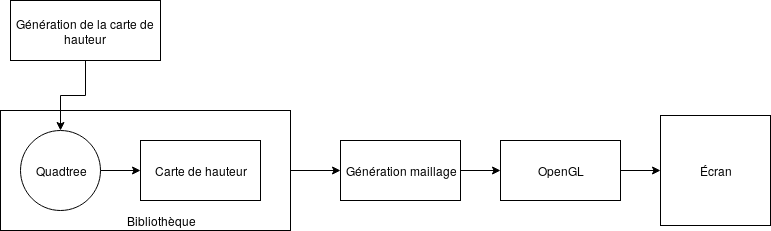
\includegraphics[scale=0.5]{img/DecoupageTache.png}
  \caption{Découpage des tâches}
  \label{fig:tache}
\end{figure}
\end{center}

Comme montré dans la figure \ref{fig:tache}, le projet peut être découpé
en quatre grandes parties.  Chaque partie est indépendante et
parallélisable. Chaque tâche peut aussi être divisée, le diagramme de
Gantt ci-contre (figure \ref{fig:gantt}) montre la répartition précise
des tâche ainsi qu'un découpage du projet en fonction du temps.

\begin{center}
\begin{figure}[!h]
  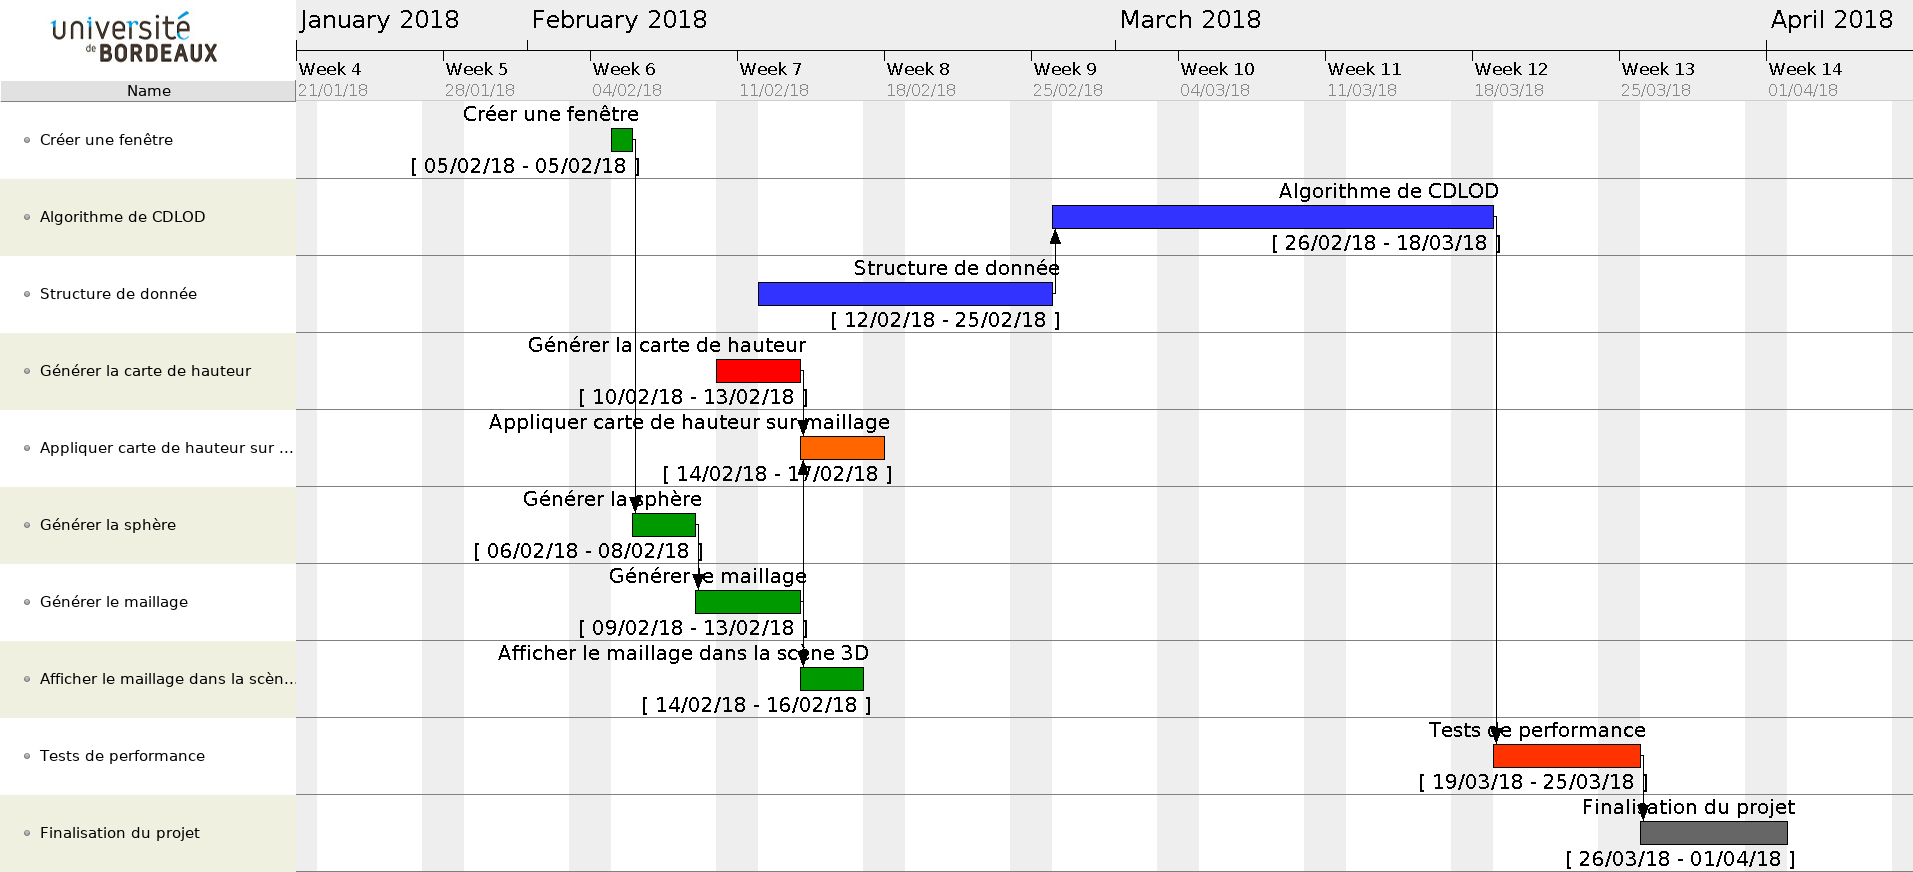
\includegraphics[scale=0.25]{img/gantt.png}
  \caption{Diagramme de Gantt}
  \label{fig:gantt}
\end{figure}
\end{center}

\bibliography{biblio}{}
\bibliographystyle{plainnat}


\end{document}
